% Options for packages loaded elsewhere
\PassOptionsToPackage{unicode}{hyperref}
\PassOptionsToPackage{hyphens}{url}
%
\documentclass[
]{article}
\usepackage{lmodern}
\usepackage{amssymb,amsmath}
\usepackage{ifxetex,ifluatex}
\ifnum 0\ifxetex 1\fi\ifluatex 1\fi=0 % if pdftex
  \usepackage[T1]{fontenc}
  \usepackage[utf8]{inputenc}
  \usepackage{textcomp} % provide euro and other symbols
\else % if luatex or xetex
  \usepackage{unicode-math}
  \defaultfontfeatures{Scale=MatchLowercase}
  \defaultfontfeatures[\rmfamily]{Ligatures=TeX,Scale=1}
\fi
% Use upquote if available, for straight quotes in verbatim environments
\IfFileExists{upquote.sty}{\usepackage{upquote}}{}
\IfFileExists{microtype.sty}{% use microtype if available
  \usepackage[]{microtype}
  \UseMicrotypeSet[protrusion]{basicmath} % disable protrusion for tt fonts
}{}
\makeatletter
\@ifundefined{KOMAClassName}{% if non-KOMA class
  \IfFileExists{parskip.sty}{%
    \usepackage{parskip}
  }{% else
    \setlength{\parindent}{0pt}
    \setlength{\parskip}{6pt plus 2pt minus 1pt}}
}{% if KOMA class
  \KOMAoptions{parskip=half}}
\makeatother
\usepackage{xcolor}
\IfFileExists{xurl.sty}{\usepackage{xurl}}{} % add URL line breaks if available
\IfFileExists{bookmark.sty}{\usepackage{bookmark}}{\usepackage{hyperref}}
\hypersetup{
  pdftitle={linear norm plot},
  pdfauthor={Joshua},
  hidelinks,
  pdfcreator={LaTeX via pandoc}}
\urlstyle{same} % disable monospaced font for URLs
\usepackage[margin=1in]{geometry}
\usepackage{graphicx,grffile}
\makeatletter
\def\maxwidth{\ifdim\Gin@nat@width>\linewidth\linewidth\else\Gin@nat@width\fi}
\def\maxheight{\ifdim\Gin@nat@height>\textheight\textheight\else\Gin@nat@height\fi}
\makeatother
% Scale images if necessary, so that they will not overflow the page
% margins by default, and it is still possible to overwrite the defaults
% using explicit options in \includegraphics[width, height, ...]{}
\setkeys{Gin}{width=\maxwidth,height=\maxheight,keepaspectratio}
% Set default figure placement to htbp
\makeatletter
\def\fps@figure{htbp}
\makeatother
\setlength{\emergencystretch}{3em} % prevent overfull lines
\providecommand{\tightlist}{%
  \setlength{\itemsep}{0pt}\setlength{\parskip}{0pt}}
\setcounter{secnumdepth}{-\maxdimen} % remove section numbering
\usepackage{booktabs}
\usepackage{longtable}
\usepackage{array}
\usepackage{multirow}
\usepackage{wrapfig}
\usepackage{float}
\usepackage{colortbl}
\usepackage{pdflscape}
\usepackage{tabu}
\usepackage{threeparttable}
\usepackage{threeparttablex}
\usepackage[normalem]{ulem}
\usepackage{makecell}
\usepackage{xcolor}

\title{linear norm plot}
\author{Joshua}
\date{15/05/2020}

\begin{document}
\maketitle

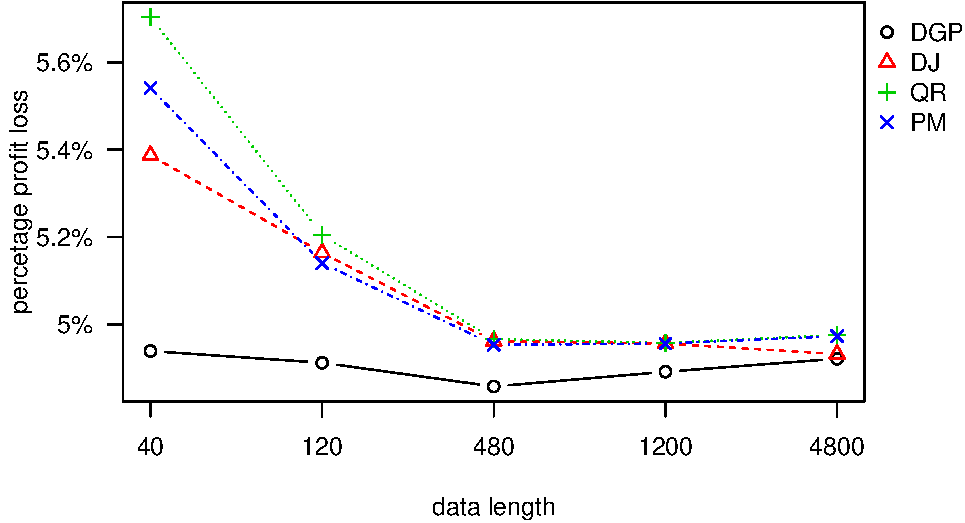
\includegraphics{linear-norm-plot_files/figure-latex/ppl0.5-1.pdf}

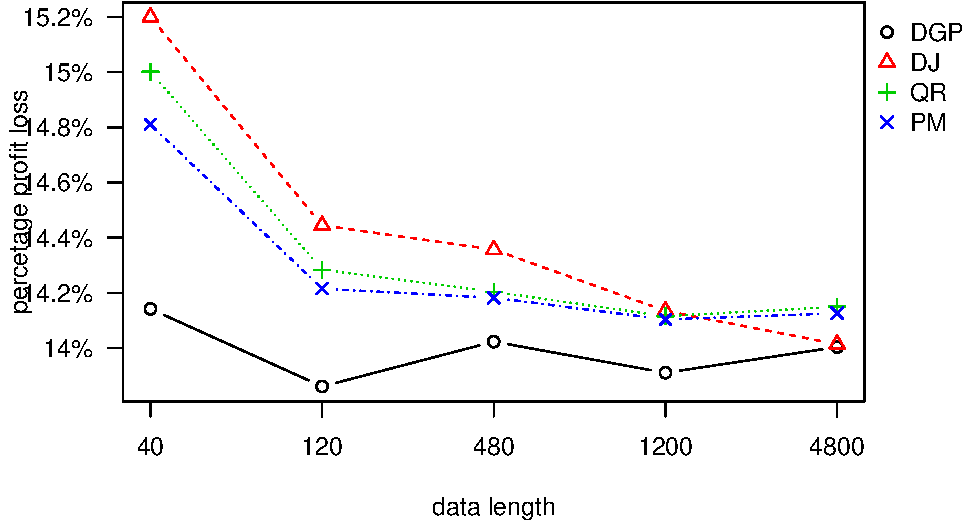
\includegraphics{linear-norm-plot_files/figure-latex/ppl0.63-1.pdf}

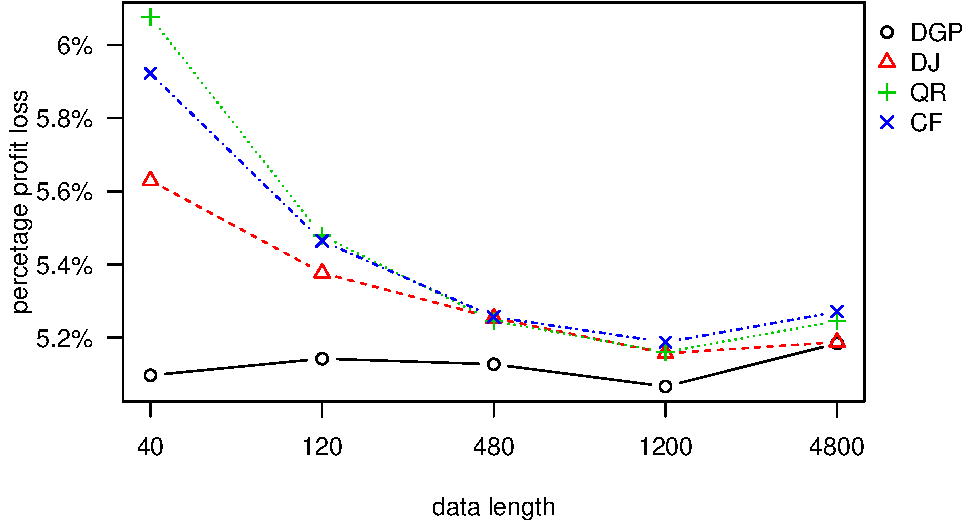
\includegraphics{linear-norm-plot_files/figure-latex/ppl0.3-1.pdf}

\begin{table}

\caption{\label{tab:inventory_error}Inventory Error}
\centering
\resizebox{\linewidth}{!}{
\begin{tabular}[t]{ccccccccccccc}
\toprule
\multicolumn{1}{c}{\textbf{ }} & \multicolumn{4}{c}{\textbf{Target service level=0.5}} & \multicolumn{4}{c}{\textbf{Target service level=0.63}} & \multicolumn{4}{c}{\textbf{Target service level=0.3}} \\
\cmidrule(l{3pt}r{3pt}){2-5} \cmidrule(l{3pt}r{3pt}){6-9} \cmidrule(l{3pt}r{3pt}){10-13}
Data size & DGP & disjoint & quantile & proposed & DGP & disjoint & quantile & proposed & DGP & disjoint & quantile & proposed\\
\midrule
\rowcolor{gray!6}  40 & 1.99 & 34.09 & 1.77 & 1.8 & -87.26 & -44.73 & -58.01 & -60.16 & 135.95 & 151.65 & 107.54 & 96.34\\
 & (200.66) & (222.63) & (233.39) & (226.28) & (199.72) & (221) & (233.15) & (224.07) & (200.51) & (223.65) & (236.36) & (227.96)\\
\rowcolor{gray!6}  120 & 1.61 & 14.04 & 1.92 & 1.58 & -76.12 & -61.38 & -70.2 & -67.3 & 115.28 & 125.84 & 107.83 & 102.9\\
 & (200.56) & (212.8) & (212.98) & (210.31) & (198.48) & (209.98) & (209.11) & (207.2) & (200.07) & (211.26) & (212.48) & (209.84)\\
\rowcolor{gray!6}  480 & 0.47 & 3.17 & 0.59 & 0.6 & -71.02 & -68.82 & -70.1 & -68.51 & 107.98 & 112.69 & 106.75 & 104.49\\
\addlinespace
 & (198.72) & (204.03) & (203.36) & (202.68) & (200.36) & (206.53) & (205.13) & (204.73) & (199.38) & (205.06) & (204.3) & (204.23)\\
\rowcolor{gray!6}  1200 & -2.38 & -0.47 & -2.48 & -2.5 & -70.72 & -70.91 & -71.07 & -69.76 & 105.82 & 109.25 & 106.58 & 104.52\\
 & (199.39) & (203.18) & (202.09) & (202.03) & (199.34) & (203.33) & (202.4) & (202.48) & (199.16) & (203.65) & (202.63) & (202.71)\\
\rowcolor{gray!6}  4800 & -1.55 & -1.16 & -1.56 & -1.54 & -70.97 & -70.85 & -71.33 & -70.19 & 104.47 & 104.92 & 105.5 & 103.93\\
 & (200.29) & (200.87) & (202.44) & (202.35) & (200.37) & (200.67) & (202.96) & (202.96) & (200.04) & (200.5) & (202.81) & (203.12)\\
\bottomrule
\end{tabular}}
\end{table}

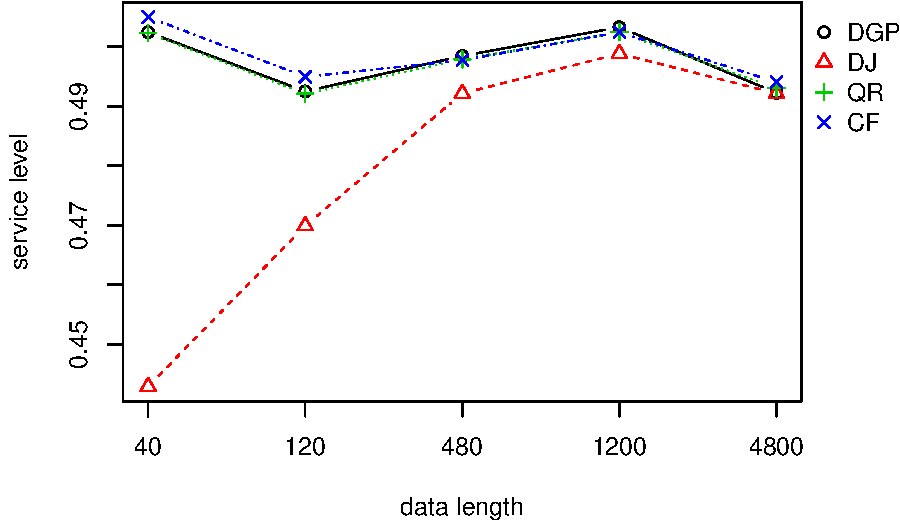
\includegraphics{linear-norm-plot_files/figure-latex/sl-1.pdf}
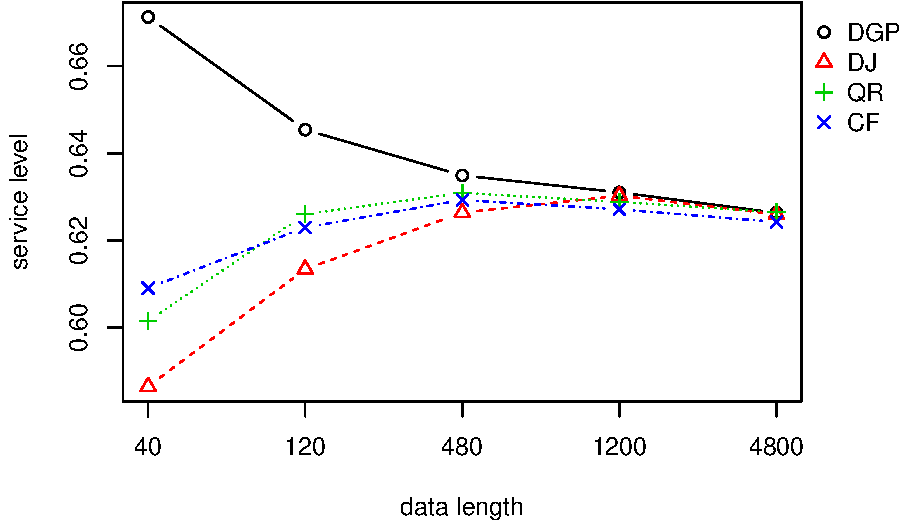
\includegraphics{linear-norm-plot_files/figure-latex/sl-2.pdf}
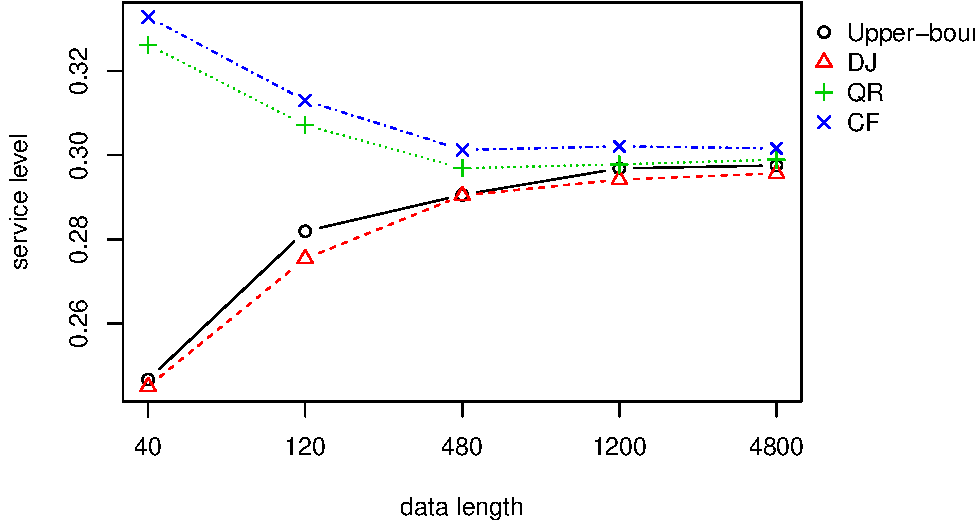
\includegraphics{linear-norm-plot_files/figure-latex/sl-3.pdf}
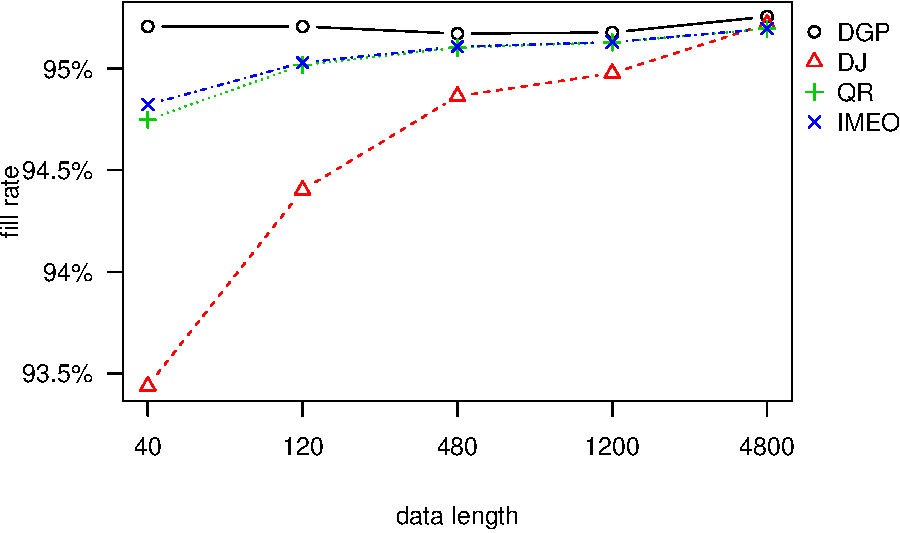
\includegraphics{linear-norm-plot_files/figure-latex/fr-1.pdf}
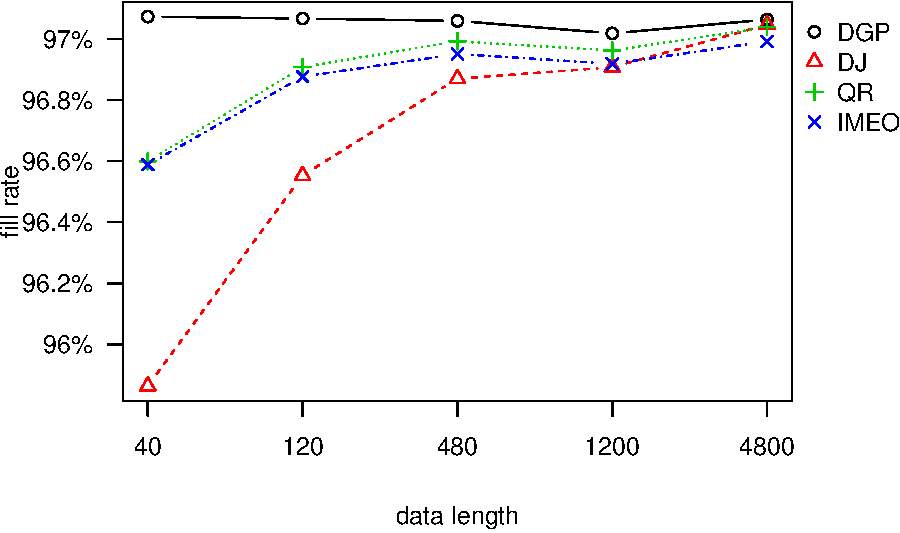
\includegraphics{linear-norm-plot_files/figure-latex/fr-2.pdf}
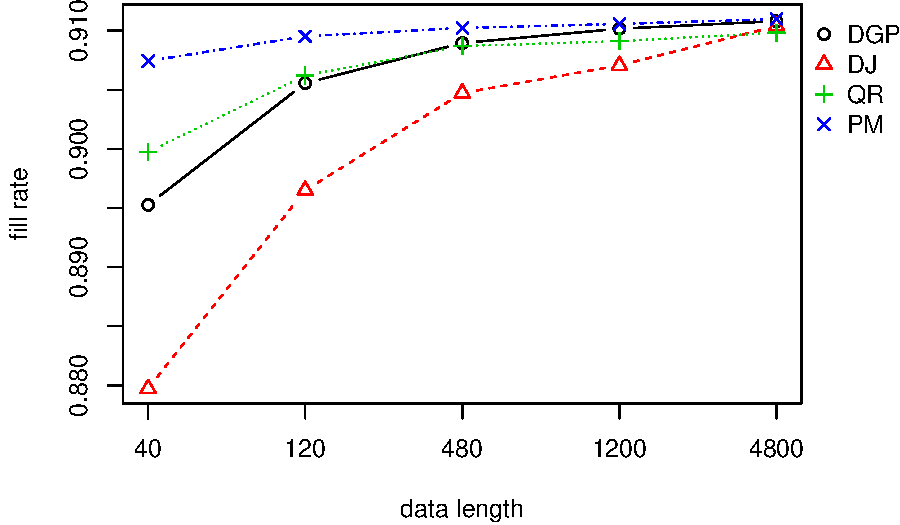
\includegraphics{linear-norm-plot_files/figure-latex/fr-3.pdf}

\begin{table}

\caption{\label{tab:Wilcoxon}p-value of Wilcoxon Test between data size 1200 and 4800}
\centering
\begin{tabular}[t]{ccccc}
\toprule
Target service level & DGP & disjoint & quantile & proposed\\
\midrule
\rowcolor{gray!6}  0.5 & 0.9760663 & 0.5352529 & 0.6818003 & 0.9920214\\
0.63 & 0.4985604 & 0.7551821 & 0.3542025 & 0.4172805\\
\rowcolor{gray!6}  0.3 & 0.3694827 & 0.3811101 & 0.7433179 & 0.9046018\\
\bottomrule
\end{tabular}
\end{table}

\textbackslash begin\{table\}

\textbackslash caption\{\label{tab:size0.3}Size effect (q=30\%)\}
\centering \resizebox{\linewidth}{!}{
\begin{tabular}[t]{ccccccccccccc}
\toprule
\multicolumn{1}{c}{\textbf{ }} & \multicolumn{4}{c}{\textbf{Percentage profit loss}} & \multicolumn{4}{c}{\textbf{Service level}} & \multicolumn{4}{c}{\textbf{Fill rate}} \\
\cmidrule(l{3pt}r{3pt}){2-5} \cmidrule(l{3pt}r{3pt}){6-9} \cmidrule(l{3pt}r{3pt}){10-13}
Data size & DGP & disjoint & quantile & proposed & DGP & disjoint & quantile & proposed & DGP & disjoint & quantile & proposed\\
\midrule
40 & 5.1\% & 5.7\% & 6.1\% & 5.9\% & 0.25 & 0.25 & 0.32 & 0.34 & 89.5\% & 88.0\% & 90.0\% & 90.7\%\\
120 & 5.1\% & 5.4\% & 5.5\% & 5.4\% & 0.28 & 0.27 & 0.31 & 0.31 & 90.6\% & 89.7\% & 90.6\% & 91.0\%\\
480 & 5.2\% & 5.3\% & 5.3\% & 5.3\% & 0.29 & 0.29 & 0.30 & 0.30 & 90.9\% & 90.5\% & 90.9\% & 91.0\%\\
1200 & 5.1\% & 5.2\% & 5.2\% & 5.3\% & 0.29 & 0.29 & 0.30 & 0.30 & 91.0\% & 90.7\% & 90.9\% & 91.1\%\\
4800 & 5.2\% & 5.2\% & 5.2\% & 5.3\% & 0.30 & 0.30 & 0.30 & 0.30 & 91.1\% & 91.0\% & 91.0\% & 91.1\%\\
\bottomrule
\end{tabular}} \textbackslash end\{table\}

\begin{table}

\caption{\label{tab:level40}Target service level effect (n=40)}
\centering
\resizebox{\linewidth}{!}{
\begin{tabular}[t]{ccccccccc}
\toprule
\multicolumn{1}{c}{\textbf{ }} & \multicolumn{4}{c}{\textbf{Percentage profit loss}} & \multicolumn{4}{c}{\textbf{Service level}} \\
\cmidrule(l{3pt}r{3pt}){2-5} \cmidrule(l{3pt}r{3pt}){6-9}
Target service level & DGP & disjoint & quantile & proposed & DGP & disjoint & quantile & proposed\\
\midrule
\rowcolor{gray!6}  0.5 & 4.9\% & 5.4\% & 5.7\% & 5.5\% & 0.50 & 0.44 & 0.50 & 0.50\\
0.63 & 14.1\% & 15.1\% & 16.0\% & 15.4\% & 0.67 & 0.58 & 0.60 & 0.60\\
\rowcolor{gray!6}  0.3 & 5.1\% & 5.7\% & 6.1\% & 5.9\% & 0.25 & 0.25 & 0.32 & 0.34\\
\bottomrule
\end{tabular}}
\end{table}

\begin{table}

\caption{\label{tab:level480}Target service level effect (n=480)}
\centering
\resizebox{\linewidth}{!}{
\begin{tabular}[t]{ccccccccc}
\toprule
\multicolumn{1}{c}{\textbf{ }} & \multicolumn{4}{c}{\textbf{Percentage profit loss}} & \multicolumn{4}{c}{\textbf{Service level}} \\
\cmidrule(l{3pt}r{3pt}){2-5} \cmidrule(l{3pt}r{3pt}){6-9}
Target service level & DGP & disjoint & quantile & proposed & DGP & disjoint & quantile & proposed\\
\midrule
\rowcolor{gray!6}  0.5 & 4.9\% & 5.0\% & 5.0\% & 5.0\% & 0.50 & 0.50 & 0.50 & 0.50\\
0.63 & 13.9\% & 14.3\% & 14.3\% & 14.2\% & 0.64 & 0.63 & 0.63 & 0.63\\
\rowcolor{gray!6}  0.3 & 5.2\% & 5.3\% & 5.3\% & 5.3\% & 0.29 & 0.29 & 0.30 & 0.30\\
\bottomrule
\end{tabular}}
\end{table}

\begin{table}

\caption{\label{tab:level4800}Target service level effect (n=4800)}
\centering
\resizebox{\linewidth}{!}{
\begin{tabular}[t]{ccccccccc}
\toprule
\multicolumn{1}{c}{\textbf{ }} & \multicolumn{4}{c}{\textbf{Percentage profit loss}} & \multicolumn{4}{c}{\textbf{Service level}} \\
\cmidrule(l{3pt}r{3pt}){2-5} \cmidrule(l{3pt}r{3pt}){6-9}
Target service level & DGP & disjoint & quantile & proposed & DGP & disjoint & quantile & proposed\\
\midrule
\rowcolor{gray!6}  0.5 & 4.9\% & 4.9\% & 5.0\% & 5.0\% & 0.51 & 0.51 & 0.51 & 0.51\\
0.63 & 14.0\% & 14.0\% & 14.2\% & 14.1\% & 0.64 & 0.64 & 0.64 & 0.64\\
\rowcolor{gray!6}  0.3 & 5.2\% & 5.2\% & 5.2\% & 5.3\% & 0.30 & 0.30 & 0.30 & 0.30\\
\bottomrule
\end{tabular}}
\end{table}

\end{document}
